%%%%%%%%%%%%%%%%%%%%%%%%%%%%%%%%%%%%%%%%%%%%%%%%%%%%%%%%%%%%%%%%%%%%%%%%%%%%%%%%
%2345678901234567890123456789012345678901234567890123456789012345678901234567890
%        1         2         3         4         5         6         7         8

\documentclass[letterpaper, 10 pt, conference]{ieeeconf}  % Comment this line out if you need a4paper

%\documentclass[a4paper, 10pt, conference]{ieeeconf}      % Use this line for a4 paper

\IEEEoverridecommandlockouts                              % This command is only needed if 
                                                          % you want to use the \thanks command

\overrideIEEEmargins                                      % Needed to meet printer requirements.

% See the \addtolength command later in the file to balance the column lengths
% on the last page of the document

% The following packages can be found on http:\\www.ctan.org
%\usepackage{graphics} % for pdf, bitmapped graphics files
%\usepackage{epsfig} % for postscript graphics files
%\usepackage{mathptmx} % assumes new font selection scheme installed
%\usepackage{times} % assumes new font selection scheme installed
%\usepackage{amsmath} % assumes amsmath package installed
%\usepackage{amssymb}  % assumes amsmath package installed

\usepackage{graphicx}
\usepackage{verbatim}

\title{\LARGE \bf
PATH PLANNING FOR MUSICAL ROBOT
}


%\author{Harrison English$^1$, Minwei Gu$^2$, David Zhang$^3$, and Yuxi Zhang$^4$
%\thanks{$^{1}$ Harrison English is with College of Computing, Georgia Institute of Technology, 
%		Atlanta, Georgia
%        {\tt\small henglish3@gatech.edu}}
%\thanks{$^{2}$ Minwei Gu is with Center of Music Technology, Georgia Institute of Technology, 
%		Atlanta, Georgia
%        {\tt\small Minwei\textunderscore Gu@gatech.edu}}
%\thanks{$^{3}$David Zhang is with College of Computing, Georgia Institute of Technology, 
%		Atlanta, Georgia
%        {\tt\small dzhang61@gatech.edu}}
%\thanks{$^{4}$Yuxi Zhang is with Center of Music Technology, Georgia Institute of Technology, 
%		Atlanta, Georgia
%        {\tt\small yzhang453@gatech.edu}}
%\thanks{$^{2}$Bernard D. Researcheris with the Department of Electrical Engineering, Wright State University,
%        Dayton, OH 45435, USA
%        {\tt\small b.d.researcher@ieee.org}}%
%}

\author{
\authorblockN{David Zhang}
\authorblockA{
College of Computing\\
Georgia Institute of Technology\\
Email: dzhang61@gatech.edu}\\
\authorblockN{Minwei Gu}
\authorblockA{
Center for Music Technology\\
Georgia Institute of Technology\\
Email: Minwei\textunderscore Gu@gatech.edu}\\
\and
\authorblockN{Yuxi Zhang}
\authorblockA{
Center for Music Technology\\
Georgia Institute of Technology\\
Email: yzhang453@gatech.edu}\\
\authorblockN{Harrison Englis}
\authorblockA{
College of Computing\\
Georgia Institute of Technology\\
Email: henglish3@gatech.edu}\\
}

\begin{document}



\maketitle
\thispagestyle{empty}
\pagestyle{empty}


%%%%%%%%%%%%%%%%%%%%%%%%%%%%%%%%%%%%%%%%%%%%%%%%%%%%%%%%%%%%%%%%%%%%%%%%%%%%%%%%
\begin{abstract}

\textit{Shimon} is an interactive robotic marimba player, developed as part of our ongoing research in Robotic Musicianship.  We discuss the robot's current constraints at playing whole piece music by itself.  We then present an planner that will reduce the note loss by intelligently planning out the positions of the four arms before beginning to play.  This planner's goal is to minimize the total global distance travelled of four arms.

\end{abstract}


%%%%%%%%%%%%%%%%%%%%%%%%%%%%%%%%%%%%%%%%%%%%%%%%%%%%%%%%%%%%%%%%%%%%%%%%%%%%%%%%
\section{INTRODUCTION}

Shimon, an interactive robotic marimba player, currently listens to a human musician and continuously adapts its improvisation and choreography, while playing simultaneously with the human.  Although currently Shimon is adept at playing improvisations it struggles playing entire pieces of written music by itself.  This paper describes a new planning algorithm for Shimon.  

We designed this planning algorithm to minimize the total distance travelled by four arms.  In doing so we will increase the ability of Shimon to play correct notes when playing pieces of written music. We reviewed previous studies in gradient descent, planners, and chess algorithms.  We adapted these algorithms in order to limit the massive branching problems that occurs with a state space of this size. We use these previous studies to derive two algorithms. One based on gradient descent and one based on limiting search.  These algorithms were implemented using \textit{JavaScript}.

\begin{figure}[h!]
\centering
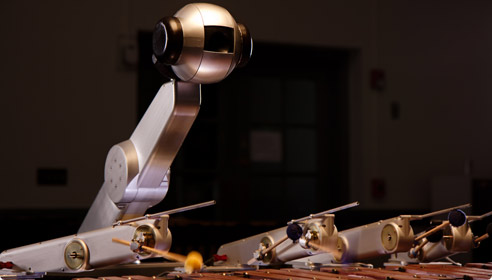
\includegraphics[scale=0.5]{Shimon.jpg}
\caption{Shimon robotic musician}
\label{Shimon}
\end{figure}

Finally we tested this planning algorithm using two songs \textit{``Ramblin''} and \textit{``For Elise''}.  Although we were unable to ascertain any empirical data showing the improvements from the planning algorithm, the planned path played notes that Shimon could not previously play or play correct with less distance travelled.  This new planned path made a distinguishable difference in performance.  In order to properly tackle this problem we will look at related works of robots in the musical field as well as some basic algorithm for gradient descent and Chess AI.


\section{RELATED WORK}

For years here in Georgia Tech Center for Music Technology, research has been focused on how to create meaningful and inspiring musical interaction with humans which leads to novel musical experiences and outcomes. The robot combines computational modelling of music perception, interaction and improvisation, with the capacity to produce melodic acoustic responses in physical \cite{HofWei10} and visual \cite{Weinberg11} manners. 

However, we have never conducted any research corresponding to the path planning of the Marimba robot. The control of the note playing is based on several high level rule, which is:

\begin{itemize}
	\item[1)] When a note is parsed for playing, the nearest arm to the location of the note is called to reach that position.
	\item[2)] If the space of the note to be played is dominated by another arm. Shimon will find its corresponding octave note to play as an alternative.
	\item[3)] If either octave doesn't work or it is just not reachable, Shimon will drop that note and go to the next. 
\end{itemize}

Two algorithms have been taken into consideration in our path planning for Shimon. Gradient descent is widely used in robotics path planning, which proves to be an efficient algorithm to find local minima.  Oke G et al. \cite{OkeIst01} implemented gradient descent to minimize the tip position error offline for the trajectory planning of a two-link robotic arm.  Soriano. L et al. \cite{MarCha08} addressed a navigation and coordination methods that allow swarms of robots to converge and spread along complex 2D shapes in environments containing unknown obstacles by using gradient descent to control the swarm.	
			
The fundamental idea of chess artificial intelligence algorithm is to design an algorithm that can play chess autonomously without human guidance. The features we took advantage of in the Chess Algorithm here were its limited branching factor and search depth.  Back to 1992, Barraquand \cite{BarLanLat92} stated that the local methods for path planning, unlikely to the traditional global graph search, is a useful way to reduce computational complexity and thus can construct potential fields numerically instead of analytically. Pivtoraiko ed \cite{PivKel05} proposed an approach to constrained path planning that is based on a special search space which efficiently encodes feasible paths. The paths are encoded implicitly as connections between states, but only feasible and local connections are included. 

We will implement our algorithms for Shimon's path planning based on the idea of gradient descent and limited search. More details will be described in the methodology section.

\section{METHODOLOGY}

\subsection{Problem Definition}

Let $p_{ik}$ be the position of arm $i$ at time $k$. (Here time is discrete value corresponding to the midi note time signature). The system takes MIDI file as input, parse it line by line to generate note sequences with midi note, velocity and duration as entries. Each time at most 4 notes can be played simultaneously. The $n$ by 5 midi matrix is fed into the system. The search algorithm will find a path that optimizes the goal function and satisfies the three types of constraints. The output sequence is a $m$ by 9 matrix, four arm positions, four velocity values for each arm, and note duration. The velocity value of 0 means that the arm just moves to that position without hitting that note. The output sequence is exported to Shimon controller to play each note individually. The system structure is shown in Figure 1.

\begin{figure}[h!]
\centering
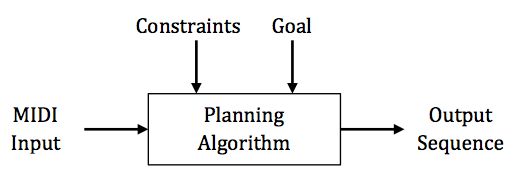
\includegraphics[scale=0.4]{figure1.png}
\caption{System Structure}
\label{System}
\end{figure}

\subsection{Constraints}

There are four cases of mechanical constraints. 

\begin{itemize}
	\item[1)] Each arm has a position range that it can reach. 
		$$\left\lbrace\begin{array}{ll}
			1 \leq p^k_1 \leq 21	&	\forall k \in [1, n]		\\
			3 \leq p^k_2 \leq 23	&	\forall k \in [1, n]		\\
			6 \leq p^k_3 \leq 26	&	\forall k \in [1, n]		\\
			8 \leq p^k_4 \leq 28	&	\forall k \in [1, n]		
		\end{array}\right.		 $$
	\item[2)] When arm 2 and arm 3 are close together, 6 notes are not reachable. 
		$$p^k_2 - p^k_3 \geq 6, \forall k \in [1, n] $$
	\item[3)] When arm 1 and arm 2 are together, or arm 3 and arm 4 are together, 2 notes will  be missing. 
		$$p^k_1 - p^k_2 \geq 2, p^k_3 - p^k_4 \geq 2,  \forall k \in [1, n] $$
	\item[4)] Each arm must follow a linear ordering.
		$$p^k_1 < p^k_2 < p^k_3 < p^k_4, \forall k \in [1, n] $$
\end{itemize}

\subsection{Goal}

The goal is to minimize the total distance traveled by four arms, represented as
	$$min\ \Sigma_{k=1}^n \Sigma_{i=1}^4 (p^k_i - p^k_{i - 1})^2$$

To achieve global minimum, we firstly explore ways to achieve local minimum for each time step, which is to calculate the minimum distance traveled to play one particular note at that time. This involves one arm to go to that position and play that node, or two arms, one moves away to make space for the second arm to go there and hit that note.	


\subsection{Algorithms}

For the robot, the state space is enormous. Because each arm can play roughly 48 notes, there are 73,815 possible configurations after accounting for the distance constraints and the linear ordering of the arms. After accounting for configurations that include the correct notes, there are still on average, approximately 6800 possible configurations. This means a song represents a branching factor for 6800 for thousands of notes. In order for a search algorithm to work, the algorithm would need to be very aggressive in pruning possible paths. To this end, we implemented two algorithms: one based on gradient descent and one based on limiting search.

The gradient descent algorithm examines all the possible ways to play the target notes from some starting position and selects the one with the smallest $L2$ norm in note distance. Because the algorithm always selects the smallest distance, there is no reason to remember any history. In a way, the algorithm is similar to a depth-first search algorithm that always picks one of the correct paths, which means backtracking is unnecessary.  The algorithm repeats this process for every note that needs to be played from each previous position.

The limited search algorithm has two parameters: search depth and branching factor. The algorithm is similar to a chess AI in that it searches a finite number of levels deep, determined by the search depth parameter. However, unlike in chess, the raw branching is in the thousands, which means even a small number of levels quickly becomes inefficient. To remedy the large branching factor, the algorithm performs a pruning similar to the gradient descent algorithm except that, instead of tossing out all but one state, the algorithm tosses out all but a finite number of states, determined by the branching factor parameter. These two parameters effectively turn an exponential search into a linear one.

The algorithms were implemented in $Node.js$, which turned out to be a rather poor choice \cite{NodeJs}. While the language is in no way slow and the potential for parallelism can make the algorithms faster, the default libraries are very poor. The only data structure that $JavaScript$ provides by default is an associative array. Notable, the associative array does not even handle indexing by other associative arrays properly. The poverty of structures means that more efficient data structures either need to be imported or built from the ground up. Almost any other popular language would have been a better choice as this poverty is a rather rare phenomenon.

Because of a lack of time, the algorithms were not optimized to a fine degree. One optimization that was implemented was a refinement on the generation of configuration states. The method used in the gradient descent algorithm simply generated all possible combinations of states that satisfied the linear ordering constraint, which meant that each note required searching through approximately 1,700,000 configurations. The refined method fixed the positions that were required and only went through all possible arm positions for arms that were free. This improved the limited search algorithm by roughly thirty percent but had no effect on the gradient search algorithm. 

\section{EXPERIMENT SETUP}

We tested two MIDI songs with our algorithm, \textit{``Ramblin''} and \textit{``For Elise''}. We use MAX/MSP for Shimon motion control, see Figure 2 for an example. In order to conveniently embed our planning algorithms into MAX, we use \textit{JavaScript} for core functionalities. The output movement script is directly fed into the control patch for Shimon to play. 

The performance shows that our planning algorithm is effective and efficient. The planned path can play notes that Shimon could not play or played wrongly before. The total distance travelled by the four arms is much less than before. Since there is no way to calculate the total distance travelled without planning, we can not quantify the distance travelled. However just based on experimental observations, there are fewer circumstances that an arm travels a long distance to play a note far away. The performance improvement is distinguishable.

\begin{figure}[h!]
\centering
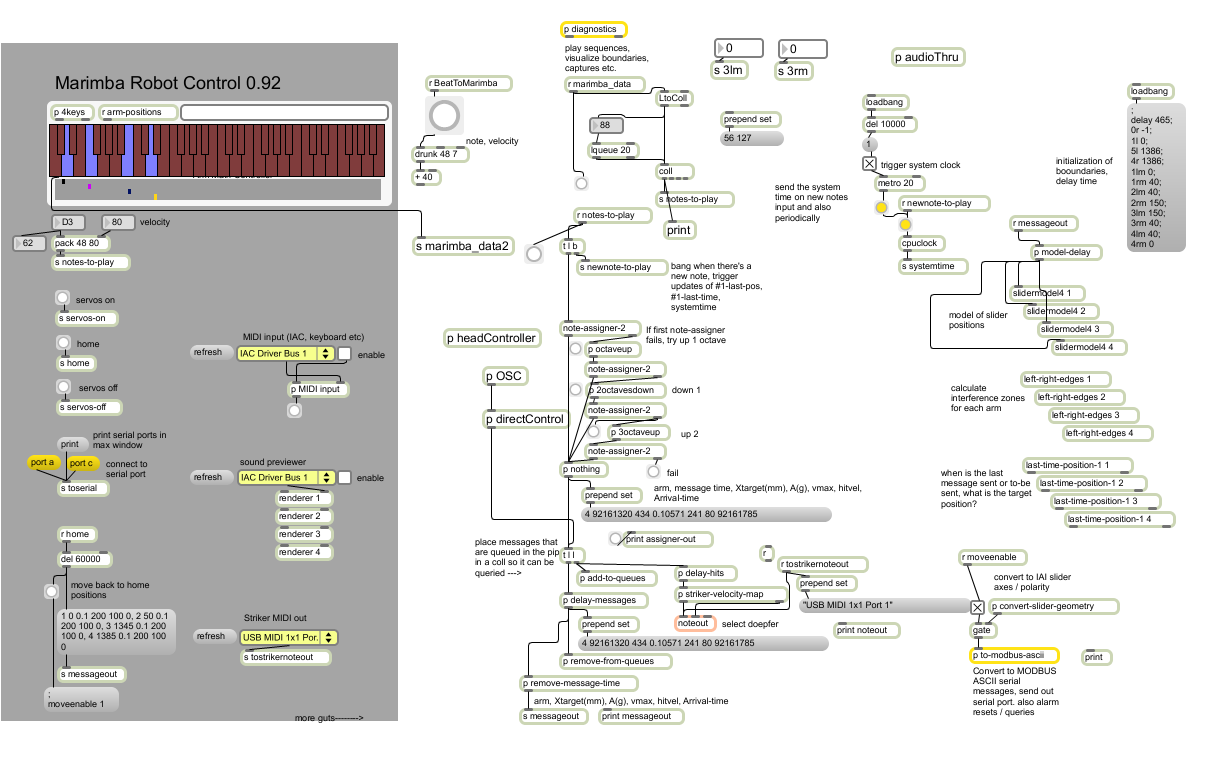
\includegraphics[scale=0.2]{figure2.png}
\caption{Shimon controller MAX patch}
\label{Max patch}
\end{figure}

\section{EVALUATION AND ANALYSIS}

\subsection{Optimality}

Because of the size of the state space, none of the algorithms perform standard search. Because none of them explore the entire state space in depth, they are partially or entirely greedy. Because they are greedy, they are not optimal. The gradient descent algorithm is entirely greedy because it looks at all possible states that can be reached from a given state and chooses the one with the lowest $L2$ cost, measured in note distance. When compared with the limited search algorithm, the non-optimality becomes clear. The limited search algorithm will produce plans where arms that are not playing notes will more towards notes that they will play in the future. The reason for this is that, while, in the short term, it is better to only move arms that need to be move, in the long term, the $L2$ norm penalizes large movements more than multiple short movements. In this sense, the gradient descent algorithm would be optimal under a $L1$ norm, but this is by condoning a certain type of sharp, high-velocity movement. While the limited search algorithm is in a sense ``more optimal'' because it looks a finite distance into the future, for efficiency reason, it cannot look far enough or branch far enough, which means it is non-optimal. The limitation is most apparent when the limited search algorithm's plan move arms toward their future positions but can not move them significantly since the branching factor was limited.

Because of the nature of songs, an optimal planner does not actually need to search through the entire song. In fact, if two adjacent chords both require four notes to be played, then there is exactly one possible and thus optimal transition. Generalizing, an optimal planner only needs to plan until all arms are used twice because only the movements between the instance of each arm being required are free to vary. This means that search depth is able to be limited, but to fully capitalize on this feature would require an analysis of a song to determine what a proper search depth should be, which could be made variable for efficiency.

Another consideration is that the effect of searching is that arm movement becomes divided into smaller steps. The type of division suggests that if the gradient descent algorithm were augmented with a path smoothing algorithm over inactive arms, then the result could be made close to optimal. The smoothing algorithm could not be as simple as linear interpolation because such an algorithm may inadvertently violate the collision constraint. Because the movements over time are in straight lines, a graph of arm positions and time would feature polygonal shapes, which means a visibility graph approach could be used for smoothing.

\subsection{Completeness}

There is a classes of songs that Shimon is not able to play. Any song that requires the collision constraint to be violated is not playable to perfection. For example, if a song requires a chord of four notes each two notes apart, then the collision constraint must be violated because the second and third arms are not able to sufficiently close. Any song with notes that are too close together in time with consideration of the specific notes. Any song that requires more than four notes where the notes are sufficiently distanced cannot be played because Shimon lacks the required number of arms. 

Even considering the classes of songs that are simply impossible to play correctly, the two algorithms are not complete. There are some situations which the algorithms fail to find a correct plan. Any song where the fact that Shimon has two drumsticks on each arm is needed will cause the algorithms to generate incorrect plans. Because the input format only allows for four notes, when such a scenario happens with more than four notes, the input format simply does not allow the song to be represented. In addition, the collision constraint is imprecise because the secondary drumsticks play sharps and flats which are one note distance away, which means such a scenario necessarily violates the collision constraint that is implemented but not the true, more complicated collision constraint. 

Any song that has a cluster of notes on one side of the marimba, a pause, and then a cluster of notes on the other side of the marimba with only small intervals for the clusters will cause the algorithms to generate incorrect plans. In this case, the plans created by the algorithms will fail because of the rarely occurring velocity constraint of the arms. This constraint is rare because there are four arms, which are always be relatively distributed over the marimba because of the collision constraint, which means the corresponding scenario is a bit specific. The plan will cause Shimon to play the first cluster, not move, then fail to move fast enough to the second cluster. A correct plan will have Shimon move during the pause, which would make the distance travelled for second cluster small enough. Note, the pause is necessary because otherwise the song is simply unplayable. This problem is solvable. For the gradient descent planner, a smoothing algorithm may move the arms sufficiently. For the limited search algorithm, an increase to the branching factor would cause the algorithm move the arms towards the second cluster. A correct solution may require that the planner takes the time into consideration such that the plan moves the arm as close as possible to the second cluster instead of halfway.

The algorithms also fails to detect all scenarios where notes are impossible to play. Specifically, if notes are impossible to play because of time constraints, then the planner will not detect this because it does not consider time.

\subsection{Efficiency}

The gradient descent algorithm is very efficient, only requiring approximately 20 milliseconds per note on a quad core processor with 4GB of RAM, which is sufficient time for the example songs if a buffer is used. The is because the time between notes for the example songs were between 8 and 1500 milliseconds with most around 300 milliseconds. However, that is at the tempo of 60 beats per minute, which is considerably slow because most songs are at 120 beats per minute. Even with half the time, most notes provide enough time for planning the next note and then a few more. Although the gradient descent algorithm was not implemented and used in an online methodology, the algorithm is efficient enough for such a usage. In terms of big-O with the number of notes in a song as $n$, the gradient descent algorithm had a run time complexity of $O(n)$. The linear runtime derives from the observation that only a finite number of operations, on order of the entire configuration space, are needed for each note. Of course, the size of the configuration space is large, but it is a constant.

The limited search algorithm is much less efficient than the gradient descent algorithm. The algorithms runtime complexity is $O(b^d n)$ where $b$ is the branching factor and $d$ is the search depth. Just as the gradient descent algorithm had a large constant factor, the limited search algorithm does as well. Theoretically, the limited search algorithm is slower by a factor of $b^{d - 1}$. In practice, for $b=5$ and $d=2$, the algorithm only took 2.5 times as long, which is half of the theoretical estimate. But for such low values of $b$ and $d$, the algorithm is relatively inefficient. However, because the algorithm was used offline, the linear order complexity means that the algorithm is still viable even with larger $b$ and $d$ values.

Some optimizations were considered but not implemented. By pre-generating the entire valid configuration space of roughly 74,000, the algorithms could iterate through a much smaller space. Another optimization would be to search through the positions that appear in a song, but this approach is tricky because the set of positions may ignore positions that are required to satisfy the collision constraint. A more limited version of this would be consider the key signature of a song to limit the space, but this suffers from the same problems as the more general version. Key signatures could be used to prioritize configuration space searching, which would allow for intelligent pruning of the configuration space search, but the efficiency gains would be limited by the need for a data structure and the added complexities in configuration iteration. Alternatively, the arms could be divided into ranges that are successively made more granular, but this also has the possibility of missing necessary positions from the collision constraint. One consideration is that, since the gradient descent algorithm is completely greedy, the algorithm can be precomputed for all pairs of valid note combinations into a rule based approach, which, unlike the original rule based algorithm, handles the collision constraint. However, pre-computation is of some but limited use for the limited search algorithm because the plans it produces may consider many branches.

\subsection{Remarks}

In the actual experiments, the robot was able to follows the plans, which means the algorithms at least work. Compared the to baseline, rule-based algorithm, the algorithms travelled less distance and lost fewer notes. Because one of the example songs \textit{``For Elise''} featured several unplayable notes, the algorithms were implemented such that they paused during those notes although there may exist more desirable behavior or ways around this such as phase shifting songs. Notably, the original rule based planner actually performs quite well, but on inspection, there is a qualitatively, noticeable difference between their performance.

\section{CONCLUSIONS AND FUTURE WORK}

An offline robotic path planning algorithm is proposed to minimize the global travelling distance of the arm and reduce the note loss before playing a specific score with the definition of constraints and problems.  Analysis and evaluation showed that the the performance is efficient and effective.

The next step contains three different direction. Firstly, we would like to try different path planning algorithms to increase the performance and reduce the computational complexity. In addition, we will modify the algorithm to make it fit more complicated pieces such as polyphonic input since right now the planner has limited support to handle polyphonic music input. Last but not least, we would like to introduce the planner to the current improvisational part to make the robot interact with human musician in a more intuitive way.

\addtolength{\textheight}{-12cm}   % This command serves to balance the column lengths
                                  % on the last page of the document manually. It shortens
                                  % the textheight of the last page by a suitable amount.
                                  % This command does not take effect until the next page
                                  % so it should come on the page before the last. Make
                                  % sure that you do not shorten the textheight too much.

%%%%%%%%%%%%%%%%%%%%%%%%%%%%%%%%%%%%%%%%%%%%%%%%%%%%%%%%%%%%%%%%%%%%%%%%%%%%%%%%



%%%%%%%%%%%%%%%%%%%%%%%%%%%%%%%%%%%%%%%%%%%%%%%%%%%%%%%%%%%%%%%%%%%%%%%%%%%%%%%%




\begin{thebibliography}{99}
\bibitem{HofWei10} Hoffman, G., Weinberg, G. (2010) ``Shimon: An Interactive Improvisational Robotic Marimba Player'' in Extended Abstracts Proceedings of International ACM Computer Human Interaction Conference (CHI 10), Atlanta, GA.
\bibitem{Weinberg11} Weinberg G. (2011), ``Gesture-based Human-Robot Jazz Improvisation'' Extended Abstract in the Proceedings of the International Conference of Machine Learning (ICML 11), Seattle, USA.
\bibitem{OkeIst01} Oke G, Istefanopulos, Y,  ``Gradient-descent based trajectory planning for regulation of a two-link flexible robotic arm'', Advanced Intelligent Mechatronics, 2001.
\bibitem{MarCha08} Marcolino L, Chaimowicz L. ``No Robot Left Behind: Coordination to Overcome Local Minima in Swarm Navigation'', Internation conference of Robitcs and Autiomation, 2008.
\bibitem{BarLanLat92} Barraquand, J, Langlois, B, Latombe, J. ``Numerical potential field techniques for robot path planning'' Systems, Man and Cybernetics, IEEE Transactions o, volume 22, 1992.
\bibitem{PivKel05} Pivtoraiko. M, Kelly.A, ``Efficient Constrained Path Planning via Search in State Lattices'', International Symposium on Artificial Intelligence, Robotics and Automation in Space, 2005.
\bibitem{NodeJs} (2013). The Node.js language. Joyent Incorporated. [Online]. Available: http://nodejs.org/.

\end{thebibliography}


\end{document}
